\section[Overview]{Overview
\footnote{
  $CVS~revision~ $Id: HacOps.tex,v 1.7 2003/11/21 18:24:31 gen Exp $ $
}
\footnote{Authors: J.Gomez \url{mailto:gomez@jlab.org}}
}


A distributed computer system
based on the 
Experimental Physics and Industrial Control System 
(EPICS)
\htmladdnormallinkfoot{}{\url{http://www.aps.anl.gov/epics}}
 architecture monitors and commands
the various Hall A systems. The basic components of the system are:
\begin{itemize}
\item Input/Output Controllers (IOCs) - VME systems containing single
board computers (SBCs) and I/O modules
(i.e analog-to-digital converters (ADCs), digital I/O and RS-232C interfaces).
Each SBC executes the real-time operating system VxWorks and the corresponding EPICS application (signal database
and sequencers).
\item Operator Interfaces (OPI) - Computers capable of executing
EPICS tools to interact with the IOCs.
The four most used tools in Hall A are (a)
a Web-enabled version of the Motif-based Display Editor/Manager (MEDM), (b) StripTool and, (c) a signal archiver.
MEDM is the main interface used for monitoring and controlling both the hall and accelerator
equipment. StripTool allows to monitor 
the behavior of one or more signals as a function of time. 
The signal archiver keeps a record of a selected set of signals.
\item Boot Servers - IOCs load the various
software components needed to perform their functions from these machines (i.e. operating system,
signal database and controls algorithms).
\item MEDM Servers - OPI computers obtain the framework of each MEDM screen from these machines.
\item Local Area Network (LAN) - the communication path joining the IOCs, OPIs and various servers.
\end{itemize}

\infolevtwo{
\section{System's Components}
Four Linux based computers are used as OPIs: hacsbc2 (Hall A counting house), hacweb1 (101B), hacweb2 (hall) and hacweb3 (101B).
Two computers act as boot servers: hacsbc2 and hlasrv (2nd-floor of counting house). Hlasrv
also acts as MEDM server. The signal archiver resides in hacweb1.
The tasks assigned to the various IOCs are,

\begin{tabular}{r p{12.0cm}}
{\bf hallasc7} & Right HRS motion control.\\[0.5ex]
{\bf hallasc6} & e-p energy measurement system.\\[0.5ex]
{\bf hallasc18} & Left HRS motion control.\\[0.5ex]
{\bf iocha1} & Arc energy measurement system - beam position and profile wire
scanners.\\[0.5ex]
{\bf iocha2} & Arc energy measurement system - 9th magnet $\int Bdl$ measurement.\\[0.5ex]
{\bf iocha3} & RICH counter. \\[0.5ex]
{\bf iocha4} & Electron detector stack - VDCs high voltage and discriminator thresholds, reset lines to various DAQ crates.\\[0.5ex]
{\bf iocha5} & Beam current monitors.\\[0.5ex]
{\bf iocha11} & Hadron detector stack - VDCs high volatge and discriminator thresholds, reset lines to various DAQ crates.\\[0.5ex]
{\bf iocha14} & Left HRS - Q2, Q3 and Dipole power supplies and cryogenics, magnetic field probes and, collimator.\\[0.5ex]
{\bf iocha16} & Right HRS - Q2, Q3 and Dipole power supplies and cryogenics, magnetic field proves and, collimator. \\[0.5ex]
{\bf iocha17} & Monitors supply of various gasses to tracking chambers.\\[0.5ex]
{\bf iocha22} & Electron detector stack - LeCroy high voltage supplies located at
various points in the hall
(i.e. beam-line and both electron and hadron detector stacks).\\[0.5ex]
{\bf iocha26} & \\[0.5ex]
{\bf iocha48} & Left and Right HRS Q1 power supplies. BigBox power supply.\\[0.5ex]
{\bf iocha49} & Septum magnets
\end{tabular}
}

\infolevthree{
\section{Operating Procedures}
Log into the Hall A control system through one of
the computers hacsbc2, hacweb1, hacweb2 or hacweb3. The task bar has a
``tool box'' icon with a small arrow on top. Clicking on the arrow brings up a 
menu. In the case of hacsbc2, the menu contains the Alarm Handler
application and three further sub-menus: Spectrometer Motion, StripTool and WebMedm.
The Alarm Handler application is not available in hacweb1 - hacweb3.
Three applications are located under Spectrometer Motion (HRS Floor Marks, LEFT HRS and RIGHT HRS),
two under SripTool (Strip Tool and Snapshot) and, three under WebMedm (Accelerator Menu,
Cryogenics Menu and Hall A Menu). To start any of these applications, use the left mouse button
to click on the application name. These applications, as described below, can be started
from a terminal. In that case, type the commands given without the quotes.

\subsection{Alarm Handler}
The Alarm Handler notifies the user when either a signal being monitored
is outside some pre-defined limits or
communication with the IOC in which the signal resides has been lost.
The Alarm Handler will only detect an abnormal signal condition if
the signal is included in the Alarm Handler configuration file
and, the corresponding IOC database record is set to produce an alarm condition.

The Alarm Handler can be started from a terminal with the command ``start\_alh''.
The default configuration file is ``\~/alh/ALH-default.alhConfig''.
A detail description of the operation and configuration of this application can be found
in the Alarm Handler Users
Guide.\htmladdnormallinkfoot{}{\url{http://www.aps.anl.gov/extensions/alh/index.php}}

\subsection{HRS Floor Marks}
This application determines the floor marks and vernier readings required
to set each spectrometer to a given angle. The application can be started from a terminal
with the command ``setspec''.

\begin{figure}[htb]
\begin{center}
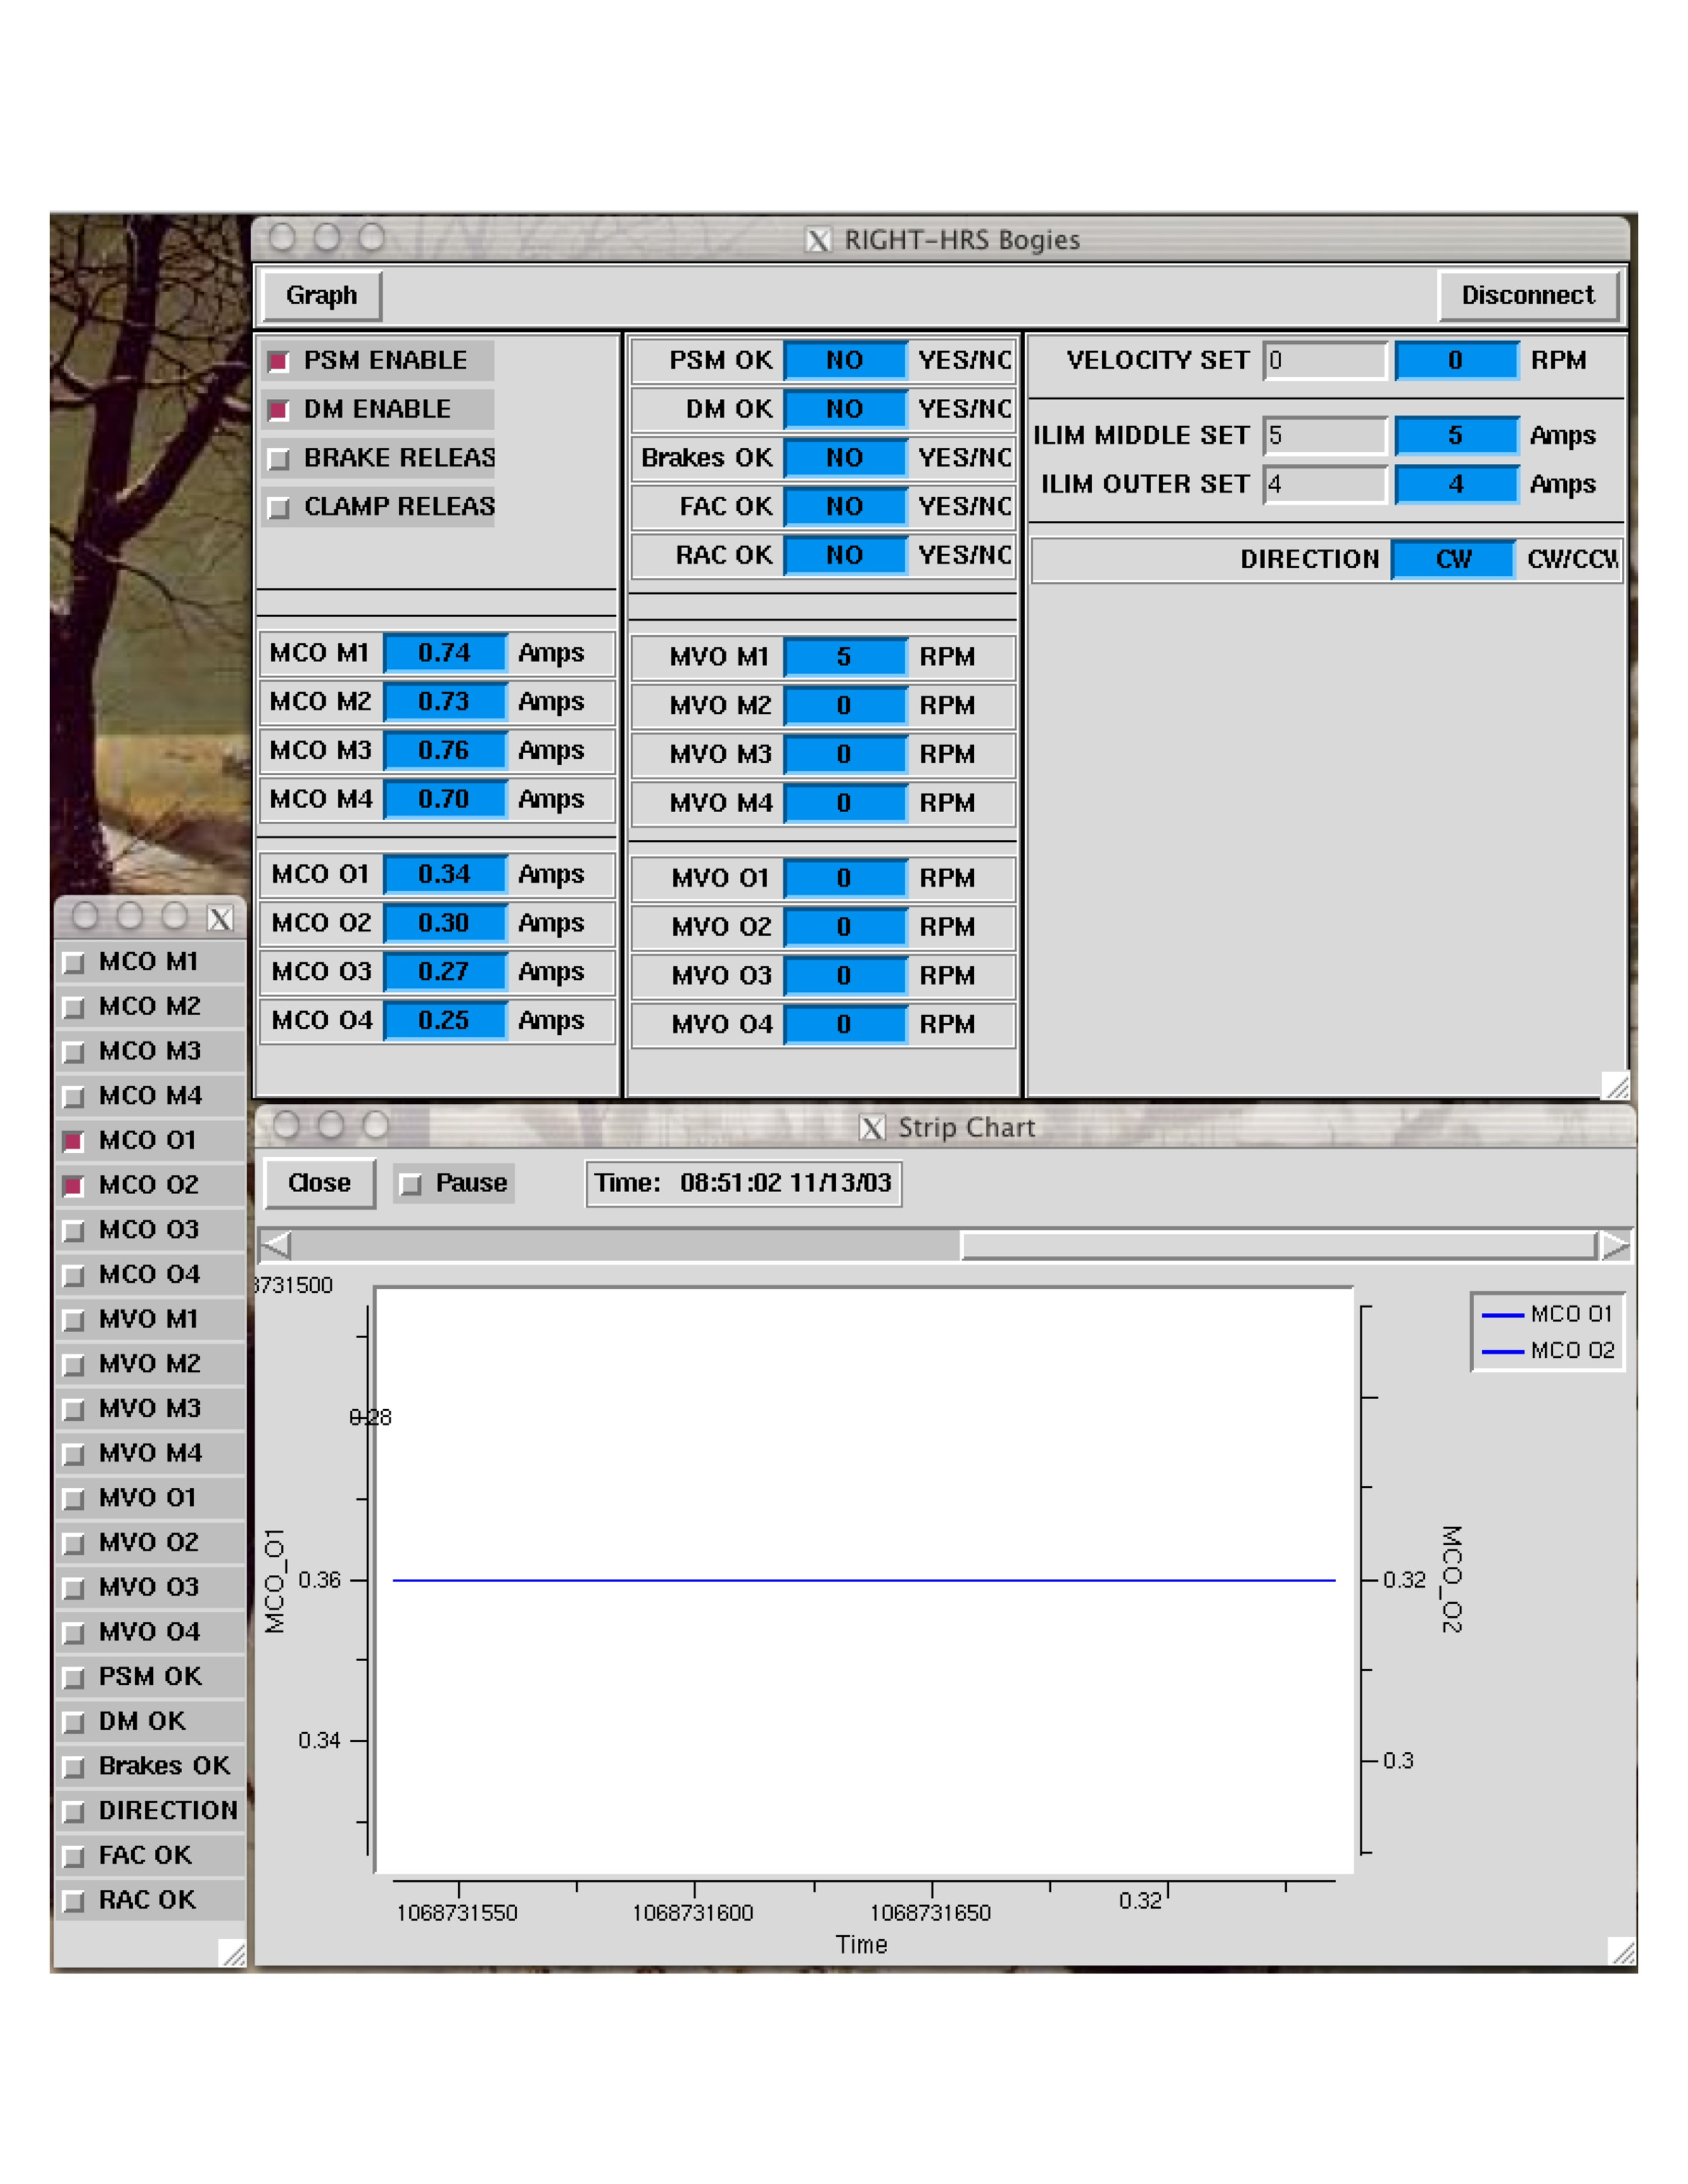
\includegraphics[angle=0,width=\textwidth]{controls-fig1}
{\linespread{1.}
\caption[Right HRS Motion Control]{Right HRS motion control.}
\label{controls-fig1}}
\end{center}
\end{figure}

\subsection{RIGHT HRS and LEFT HRS}
The ``RIGHT HRS'' (``LEFT HRS'') application is used to set the right (left)
spectrometer angle.
To start the ``RIGHT HRS'' (``LEFT HRS'')
application from a terminal type the command ``bogies\_RIGHT'' (``bogies\_LEFT'').
The ``RIGHT HRS'' and ``LEFT HRS'' applications are very similar so, we will
use ``RIGHT HRS'' as an example.

Upon starting the ``RIGHT HRS'' application, 
a screen labeled ``RIGHT-HRS Bogies'' will open as shown in
Fig. \ref{controls-fig1}.
Pressing the button labeled ``Graph'' in the top-left corner of ``RIGHT-HRS Bogies''
will open two more screens: one labeled ``Strip Chart'' and an associated, column like,
signal selection screen. The signal selection screen allows to select the signals
to be plotted in the Strip Chart screen. All signals are plotted with the same color.
To highlight a given signal,
use the plot legend located towards the right of the Strip Chart screen: clicking on the line next
to the signal name will change its color in the main plot.
The plot screens are likely to be more useful to the Hall A technical staff than to the
shift personnel.

The application screens show the Motor Current Output (MCO) and Motor Velocity Output (MVO) for each
of the four middle-ring (M1-M4) and four outer-ring (O1-O4) motors.
Also shown are the status and request buttons for the Power Supply Module (PSM),
Drive Modules (DM),
brakes and, clamps. The clamp request button (``CLAMP RELEAS'') actually releases two interlock
circuits (the Forward Amplifier Clamp or FAC and the Reverse Amplifier Clamp or RAC)
so that the spectrometer is
able to move in any direction (i.e. clockwise or counter-clockwise).
It is worth to stress that the PSM, DM, brakes and clamps request buttons represent
\underline{requests} that the hardware interlock circuits may negate. This can be clearly
seen 
in Fig. \ref{controls-fig1} which was taken with
the electrical power to the PSM and DMs disabled for septum magnet installation
in the central pivot area. Note that PSM and DM request buttons are selected (red color)
yet the corresponding status fields show interlock incomplete status (``NO'').

To move the spectrometer, select the request buttons in descending order, starting with
``PSM ENABLE'' and ending with ``CLAMP RELEAS''. After selecting a button, wait
until the corresponding status changes to ``YES''. 
If the status does not change, reboot
the IOC using the green buttons located in the middle room of the counting house.
If the failure persists, contact the Hall A on-call tech.
After the clamps have been successfully released, enter a value in the ``VELOCITY SET'' field
(see Fig. \ref{controls-fig1} - ``RIGHT-HRS Bogies'' screen). The sign of the velocity
will determine the sense of spectrometer rotation. The sense of rotation is displayed by the
field ``DIRECTION''.

\begin{safetyen}{30}{10}
Safe operation of the spectrometer motion systems requires,
\begin{itemize}
\item Find out from the shift leader the administrative constraints imposed on
spectrometer motion.
These constraints are communicated by the Hall A technical staff to the run-coordinator.
Moving the spectrometers while no experiment is taking place (for example,
a maintenance period), must first be approved by the head of the Hall A technical
staff (E. Folts) or the person designated by him.
\item If the administrative constraints allow to move the spectrometers remotely,
use the Hall A cameras
to ensure there are no objects in the path of the spectrometers.
\item Check that the floor marks are seen in the TV monitors.
\item Bring up the spectrometer motion application and go through the required steps
to get the spectrometer moving. Look at the floor marks
to ensure that the spectrometer is moving in the desired direction.
\item While the spectrometer is moving, use
the Hall A cameras to check that everything looks normal (for example, the cryogenic lines
around the pivot). If something does not look right, de-selecting ANY of the
interlocks (``PSM ENABLE'',..,``CLAMP RELEAS'') will stop the spectrometer immediately.
\item As the spectrometer approaches the desired floor mark, reduce the spectrometer
speed. De-select the ``CLAMP RELEAS'' button to stop the spectrometer at the desired floor mark.
\item De-select the remaining interlocks: ``BRAKE RELEAS'', ``DM ENABLE'' and ``PSM ENABLE''.
\item Press the button labeled ``Disconnect'' to close the spectrometer motion
application.
\end{itemize}
\end{safetyen}

\subsection{Strip Tool}
Strip Tool plots a real-time strip chart of the values of one or more signals.
It is useful to monitor data trends.

A detail description of the options and operation
of this application can be found in the Strip Tool Users
Guide\htmladdnormallinkfoot{}{\url{http://www.aps.anl.gov/extensions/StripTool/index.php}}
with one difference; the version used by Hall A does not have a ``print'' function.
To print a strip chart use the application ``Snapshot'' described below.
To start Strip Tool from a terminal type the command ``StripTool''.

\subsection{Snapshot}
Snapshot refers to a KDE desktop application (ksnapshot) which allows to grab an image
of either the whole
screen or an individual window. The image can then be sent to a printer or stored on disk.
The application can be started from a terminal with the command ``ksnapshot''.

\subsection{Accelerator Menu}
The ``Accelerator Menu'' application brings up a web-version of Monticello,
the root MEDM screen giving access to the various accelerator systems. Access to those
systems is read-only mode except for some Hall A applications which are described elsewhere
in this OSP. Not all the menus shown in this web-version of Monticello are operational
because they still are linked to directory structures residing in specific
Machine Control Center (MCC) computers. The application can be started from a terminal with
the command ``accmain''.

\subsection{Cryogenics Menu}
The ``Cryogenics Menu'' application brings up the End Station
Refrigerator (ESR) menu. Access to all ESR systems is read-only mode. This application
is typically used by the Hall A technical staff to
monitor the hall cryogenics. The application can be started from the terminal with the command ``esrmenu''.

\subsection{Hall A Menu}
The ``Hall A Menu'' application brings up a menu giving access to all the EPICS based control systems in Hall A. The application can also be started from a terminal with the command ``hlamain''.

\section{Troubleshooting Procedures}
The status of most IOCs can be seen
by opening the `Hall A Menu'' $-->$ ``IOCs''. White entries means that the IOC
is not responding which can be due to either the IOC not being used by the present
experiment or it has failed. Rebooting of the IOCs is accomplished in several ways
depending on the specific IOC. If the specific IOC can be rebooted through the
Web, the url address is given next to it. The required user and password are
posted in the Hall A Counting House. The remaining IOCs are rebooted through
either the green buttons located in the middle room of the counting house
or the crate resets screen ``Hall A Menu'' $-->$ ``Tools'' $-->$ ``Crate Resets''.

If an IOC fails to reset and its name is ``iocha..'', call MCC and request that
the software on-call person be notified. If the name is ``hallasc..'' call J. Gomez.

}

%\clearpage % forces LaTeX to finish all remaining open floats

% ===========  CVS info
% $Header: /group/halla/analysis/cvs/tex/osp/src/controls/HacOps.tex,v 1.7 2003/11/21 18:24:31 gen Exp $
% $Id: HacOps.tex,v 1.7 2003/11/21 18:24:31 gen Exp $
% $Author: gen $
% $Date: 2003/11/21 18:24:31 $
% $Name:  $
% $Locker:  $
% $Log: HacOps.tex,v $
% Revision 1.7  2003/11/21 18:24:31  gen
% polishing
%
% Revision 1.6  2003/11/16 15:15:45  gomez
% *** empty log message ***
%
% Revision 1.5  2003/11/14 22:53:00  gomez
% *** empty log message ***
%
% Revision 1.4  2003/06/06 17:19:22  gen
% Revision printout changed
%
% Revision 1.3  2003/06/06 15:31:03  gen
% Revision printout changed
%
% Revision 1.2  2003/06/05 23:30:00  gen
% Revision ID is printed in TeX
%
% Revision 1.1.1.1  2003/06/05 17:28:32  gen
% Imported from /home/gen/tex/OSP
%
%  Revision parameters to appear on the output
